\section{Empirical evaluation for sustainable data centers}
\label{sec:sustainableDataCenters}

\subsection{Experimental setup}
\label{sec:setup}

We carry out evaluation based on the settings of a HP EcoPOD data center \cite{hpEcoPODs}.

\textbf{Demand side}. The power demand capacity of the data center is 1MW. 
The power demand is from both IT equipment serving both interactive and batch workloads, and from cooling facilities removing the heat. The peak power usage is 720kW. The Peak-to-Mean Ratio (PMR) of interactive workload is set at 3. Flexible workloads (batch jobs) are 50\% of the total IT workload demand with flexibility 24 hours. The utilization of interactive workloads in a server is 40\%, and the maximum utilization for all workloads is 90\%. PUE is set at 1.2. We study the PMR and flexible workload ratios in terms of capacities and costs in Figure \ref{f.PMR} and \ref{f.batch_ratio}.

\textbf{Supply side}. We consider a power micro-grid to supply the data center. The power micro-grid consists of on-site photovoltaic (PV) array, general electric (GE) natural gas engines, and the electricity grid (grid). 

\emph{PV array:} The amortized infrastructure cost of PV array after rebate is \$2.15/W \cite{solarCost}. The maximum size of PV array is 1MW.  The operational cost and maintenance cost of PV array are respectively \$0/kWh and \$0.005/kWh. The PV capacity factor average is 18\% which is from the trace of Houston PV generation.

\emph{GE engines:} The amortized infrastructure cost of GE engines is \$1/W. Maximum size of GE engines can be installed is 1.4MW. The operational cost is \$0.06/kWh (natural gas, \$5/Mcf \cite{gasPrice}, 30\% efficiency), while the maintenance cost is \$0.005/kWh. We vary the natural gas price in Figure \ref{f.capacity_gas} to study the impacts of natural gas prices.

\emph{Electrical grid:} The base electricity price is fixed at \$0.056/kWh (Texas) \cite{electricityRateTexas}. There is no sell back price. 

\emph{Emissions:} The emissions rate from PV array, GE generation, and electricity grid are 0.034g/kWh, 0.443g/kWh, and 0.5g/kWh, respectively.

\emph{Prediction errors.} Prediction errors are assumed to be mutually independent and follow the normal distribution with zero mean. To study the impacts of prediction errors, we vary the normalized RMSEs (root mean squared errors) in Figure {\ref{f.prediction}}.

%The capacity of electricity grid is implicitly the peak of grid power consumption (grid peak).

\subsection{Optimizing traditional data centers with renewable energy}
\label{sec:Comparison}

\hideit{
\begin{figure*}[!ht]
 \begin{center}
 \subfigure[Capacities]{{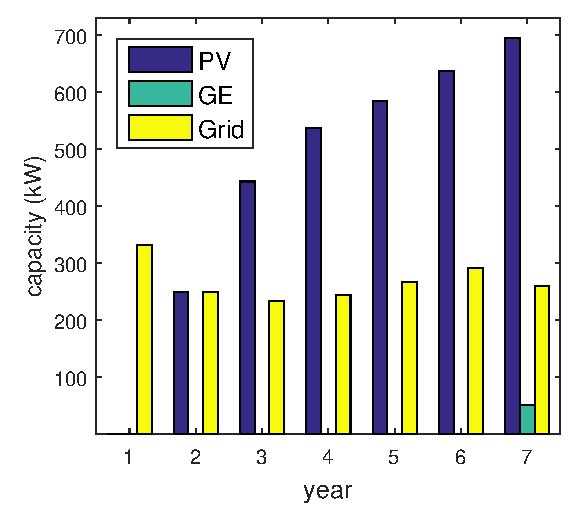
\includegraphics[width=0.32\columnwidth]{figs/long_term_capacity}}
 \label{f.capacity_annual_change}}
 \subfigure[Expenditures]{{\includegraphics[width=0.32\columnwidth]{figs/long_term_cost}}
 \label{f.cost_annual_change}}
 \subfigure[Normalized emissions]{{
\includegraphics[width=0.32\columnwidth]{figs/long_term_co2_norm}}
 \label{f.co2_annual_change}} 

 \caption{Annual capacity planning. The data center is going to use more PV generation and GE generation while reducing the imported energy from the electricity grid. The major expenditure concentrates on the infrastructure of PV. The normalized emissions go down due to the high penetration of PV generation.}
 \label{f.annual_change}
 \end{center}

\end{figure*}
}
In this subsection, we evaluate the joint framework on planning and operating a sustainable data center. We answer three questions: How does the optimization framework plan annually? How much benefits can the optimization framework achieve? How do prediction errors impact on the proposed framework?

\textbf{Annual capacity planning.} In practice, the electricity prices, gas prices, and workload demand tend to increase in the long-term. The average annual-increasing rates of electricity prices, gas prices, and workload demand are $1.05$, $1.01$, and $1.09$ \cite{eiaElectricityPrices,gasPrice,StevenGlobalTraffic}. Meanwhile, the amortized cost of PV array decreases 12\% annually \cite{solarCost}.

Figure~\ref{f.capacity_annual_change} presents the capacities of power sources in 7 years. In general, the data center increases the capacity of PV annually but not the peak grid power consumption. In the first year, the data center prefers the electricity grid to other power sources because of the low electricity price. However, the data center significantly expands PV generation capacity from year 2 as the electricity prices increase and the infrastructure cost of PV decreases. In year 7, the data center provisions GE generation since the slow natural gas becomes relatively cheaper than the imported electricity. Although the data center prefers to use PV, the peak grid power consumption is still noticeably large. The intuition behind this is that PV generation is not available during night time which requires the data center to provision grid power.

Figure~\ref{f.cost_annual_change} shows the annual breakdown expenditures of the data center. In the first year, the utility bill (Util) of the imported energy from the electricity grid is dominant. Meanwhile, the cost of PV infrastructure (PV-I) quickly increases because PV amortized cost is added by installing more PV every year. The PV O\&M (PV-O) expenditure linearly increases as the PV capacity goes up. In year 7, the GE O\&M cost (GE-O) is 15\% the total annual expenditure. GE-O mainly comes from the amount of natural gas supplied to the GE.

The annually normalized emissions of the data center, defined as the ratios of total emissions to the total power demand, are plotted in Figure~\ref{f.co2_annual_change}. Since the normalized emissions of the electricity grid are high, the normalized emissions of the data center are highest in year 1.
The increase of the PV generation can reduce normalized emissions for the data center. The normalized emissions sharply go down to 36\% in year 4 as compared to the first year. However, there is little change from year 4 to year 7 as the ratio of PV capacity to other power sources is not considerably decreased.

\hideit{
\begin{figure*}[!ht]
 \begin{center}
	 \subfigure[Grid-only (GRID)]{{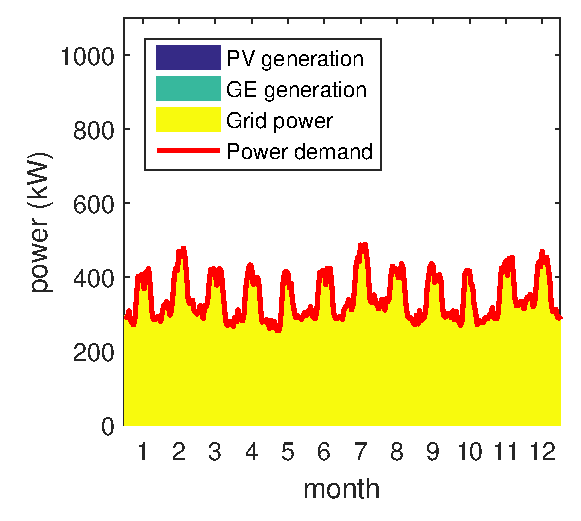
\includegraphics[width=0.32\columnwidth]{figs/nz-grid_year}}
	 \label{f.grid}}
	 \subfigure[Supply-only (SUP)]{{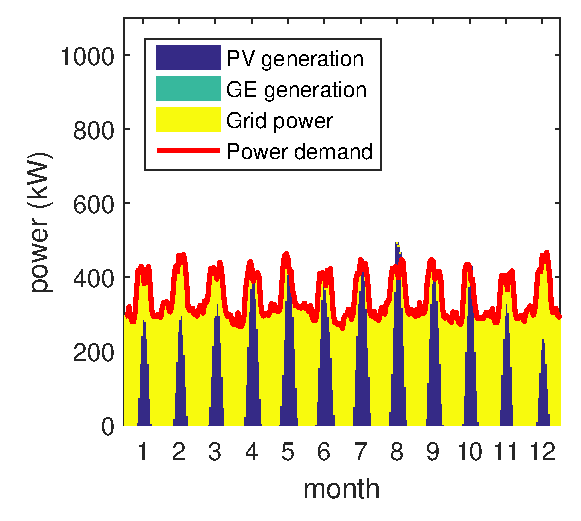
\includegraphics[width=0.32\columnwidth]{figs/nz-supply_year}}
	 \label{f.supply}}
	
	 \subfigure[Demand-only (DEM)]{{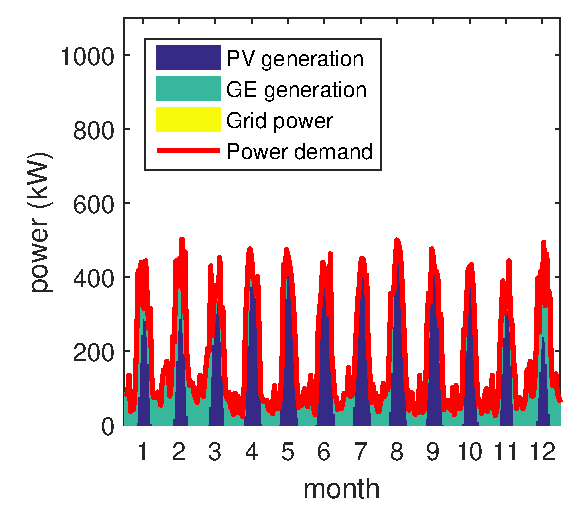
\includegraphics[width=0.32\columnwidth]{figs/nz-demand_year}}
	 \label{f.demand}}
	 \subfigure[Proposed (PROP)]{{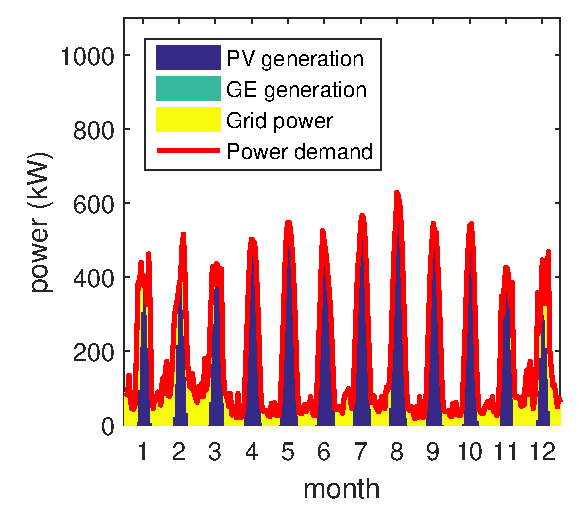
\includegraphics[width=0.32\columnwidth]{figs/nz-int_year}}
	 \label{f.integrated}}

 \caption{The power profiles of the baseline methods and the proposed framework in year 5. GRID provisions the only grid power. SUP optimizes the power sources only at the supply side. DEM optimizes the power demand, i.e., scheduling the batch jobs. } 
 \label{f.behaviors}
 \end{center} 

\end{figure*}
}

\textbf{How much cost savings and emission reductions does the proposed framework achieve?} To highlight the benefits of the proposed framework, we compare the proposed framework (PROP) with three baseline methods, namely grid-only, supply-only, and demand-only. 
\begin{itemize}

 \item Grid-only (GRID): \new{The grid-only method only uses the grid power from the electricity grid to provision the power demand. It does not use any power demand management techniques.}

 \item Supply-only (SUP): Given the power demand, the supply-only method optimizes capacity planning at the supply side.
This method can optimize the use of energy sources among PV, GE, and the public electricity grid. 

 \item Demand-only (DEM): \new{At the supply side, the capacities of PV and GE generation are set at 50\% and 70\% of the power demand capacity, respectively. 
The demand-only method optimizes the power demand, i.e., scheduling the batch jobs, to reduce the operational cost.}

\end{itemize}
In fact, PROP combines the SUP and DEM, and therefore can provide the best cost reductions.

The power profiles of these four methods in twelve typical days representing for the twelve months in year 5 are shown in Figure \ref{f.behaviors}.
GRID provisions power only from the electricity grid. SUP prefers the PV sources to the electricity grid and GE. Meanwhile, DEM utilizes installed GE generators because the electricity price is relatively more expensive than the O\&M cost of GE sources. However, PROP uses only PV generation and grid power. In Figure \ref{f.demand} and \ref{f.integrated}, DEM and PROP shape the power demand to follow the PV generation while GRID and SUP are dependent on imported electricity.
\hideit{
\begin{figure}[!th]
 \begin{center} 
 % \subfigure[Capacities]{{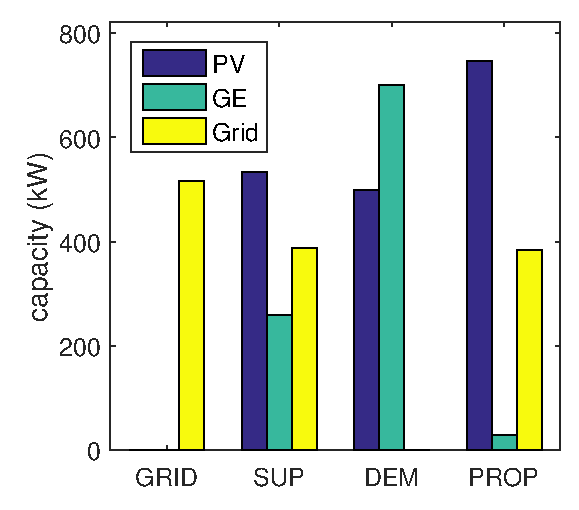
\includegraphics[width=0.48\columnwidth]{figs/capacity_comparison}}
 % \label{f.capacity_comp}}
 % \hspace{0.5cm}
 \subfigure[Expenditures]{{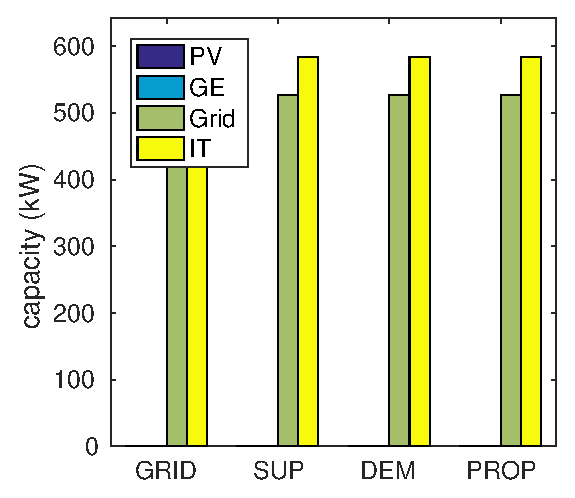
\includegraphics[width=0.32\columnwidth]{figs/cost_comparison}}
 \label{f.cost_comp}}
 % \hspace{0.5cm}
 \subfigure[Emissions]{{\includegraphics[width=0.32\columnwidth]{figs/emission_comparison}}
 \label{f.co2_comp}} 

 \caption{Comparisons with baseline methods. The proposed framework reduces up to 50\% of the total expenditures, and significantly cuts down 75\% greenhouse gas emissions.} 
 \label{f.basic}

 \end{center}
\end{figure}
}

We evaluate the four methods in terms of costs and emissions in Figure \ref{f.basic}. It shows that PROP remarkably reduces the total expenditure by 50\% while it achieves very close emissions to the lowest one, i.e., DEM. In Figure \ref{f.cost_comp}, SUP slightly reduces the total cost as it still depends much on the electricity grid. However, DEM shows that power management at demand side is very effective because it makes the power demand follow the PV generation.

\delete{\textbf{Should we provision IT capacity?} In order to highlight the importance of optimizing IT capacity, we carry out an experiment that plans the capacities of IT capacity and power sources. In Figure {\ref{f.IT}}, the IT capacities in the four methods are different. The proposed framework allows data center operators to provision the smallest IT capacity compared to other baseline methods. Consequently, the proposed framework can significantly reduce the total expenditure. Hence, the capacity of IT plays an important role reducing the total cost of ownership.}

\del{
	\begin{figure}[!htbp]
		\begin{center}
			\subfigure[Capacity]{{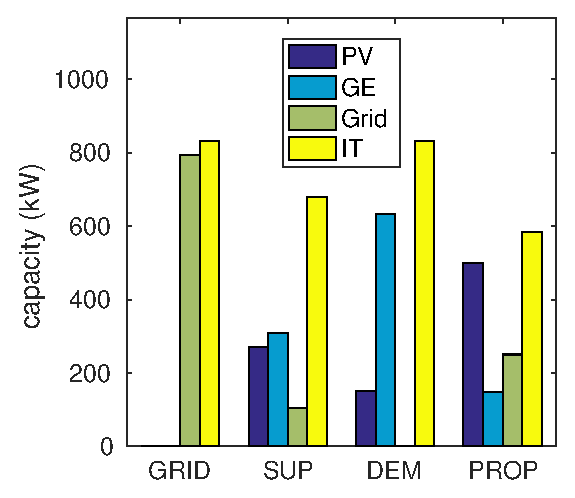
\includegraphics[width=0.48\columnwidth]{figs/capacity_IT}}
				\label{f.capacity_IT}}
			\subfigure[Cost]{{\includegraphics[width=0.48\columnwidth]{figs/cost_IT}}
				\label{f.cost_IT}}
			\caption{Comparisons with different baselines when IT capacity is also optimized. The IT capacitiy plays an important role in capacity planning.}
			\label{f.IT}
		\end{center}
	\end{figure}}


\textbf{\textit{Key insights}}: (i) The proposed framework not only remarkably reduce the total cost, but also utilizes renewable energy very well. (ii) As the renewable installation becomes more cost-effective, the proposed framework prefers to use renewable energy and reduce the dependence of sustainable data centers on the electricity grid. 
%\delete{(v) If we have opportunity to optimize IT subsystem, this can have considerate impact on the total annual expenditure of the data center.}

\subsection{Impacts of prediction errors}
\label{sec:ImpactOfPredictionErrors}

%Since the capacity planning of a data center is executed in the long-run, it suffers from prediction errors.

%To study the impact prediction errors on capacity planning
Prediction errors are generally negligible during operational management, which happens in real-time. Hence, GRID and DEM are not affected by the prediction errors because they do not need capacity planning. On the other hand, SUP and PROP suffer from prediction errors because they provide the capacity planning decisions, and then operate the data center in real-time based on the planned capacities. We normalize the root mean squared errors (RMSE) compared to the means of interactive workloads, batch jobs, capacity factors of PV, electricity prices, and gas prices, respectively. For instance, when normalized RMSEs are $0.2$, the RMSEs of all the aforementioned predictions are 20\% of their means. 

Figure {\ref{f.cost_err_comparison}} shows the impacts of prediction errors on the total expenditures of the four methods. As the prediction errors become large (more than 10\%), the total costs of SUP and PRO go up while the costs of GRID and DEM stay unchanged. Interestingly, total cost of the proposed framework is still the best and achieves the significant cost savings, i.e., 58\% of GRID. The intuition behind this is that the operational management is cost-efficient in using the various power sources and scheduling the batch jobs to compensate for the prediction errors.

The impacts of prediction errors on emissions are presented in Figure {\ref{f.emission_err_comparison}}. As the prediction errors increase, the emissions of PROP go up. However, PROP still reduces 49\% of emissions reduction compared to GRID. Specially, the emissions stay unchanged when RMSE is greater than 0.2.
%The curve of the supply-only method is more interesting. It first does not change much at normalized errors less than $0.05$, goes up from $0.05$ to $0.25$, and finally goes down as the normalized errors greater than $0.25$. Because of prediction errors, the supply-only method over-provisions the PV capacity. When the prediction errors are too small, the over-provisioned PV capacity is useful in reducing the emissions. When the normalized errors become larger, the supply-only method uses more electricity grid to compensate the renewable energy which causes more emissions. However, when the electricity prices are very unpredictable, it prefers the gas engines that release less emissions than the public electricity grid.

\hideit{
\begin{figure}[!th]
	\vspace{-0.1cm}
 \begin{center} 
 \subfigure[Expenditures]{{\includegraphics[width=0.32\columnwidth]{figs/cost_err_comparison}}
 \label{f.cost_err_comparison}} 
 \subfigure[Emissions]{{\includegraphics[width=0.32\columnwidth]{figs/emission_err_comparison}}
 \label{f.emission_err_comparison}} 
 \caption{Impacts of prediction errors. Under large prediction errors, the proposed framework still achieves the significant cost and emission reductions.} 
 \label{f.prediction}
 \end{center}
  \vspace{-0.3cm}
\end{figure}
}
\textbf{\textit{Key insights}}: Under large prediction errors, our proposed framework still achieves significant cost and emission reductions compared to the baseline methods.

\subsection{Sensitivity analysis}
\label{sec:netzero_evaluation}

We carry out the experiments based on a real data center, called Net-zero Energy Data Centers (NEDC) invented by HP \cite{arlitt2012towards}. 
In NEDC, the total local generation (i.e. PV and GE generations) is greater than the total power consumption. NEDC have an additional constraint
$$\sum_{t=1}^{T}\sum_{r=1}^{R}c_{r}(y,t) + \sum_{t=1}^{T}\sum_{s=1}^{S}c_{s}(y,t) \geq \sum_{t=1}^{T}P(y,t), \quad \forall y,$$
where the left hand side and the right hand side are the total power generation and the total power consumption in year $y$, respectively.

We focus on studying the impacts of supply and demand factors on the data centers during the first year. The supply factors include electricity price, and gas price. The demand factors include shape of interactive workload and ratio of flexible workload. Besides the capacities and expenditures of the data center, we study the payback period, which is the number of years for the data center to recoup the investment in the infrastructure costs of PV and GE instead of using only the electricity grid. The shorter payback period is, the more financial benefit the proposed framework provides.

\subsubsection{Impacts of supply factors}

\hideit{
\begin{figure}[!ht]
%matlab: TCO_grid_electricity_0115.m
\vspace{-0.1cm}
\begin{center}
	\subfigure[Capacity]{{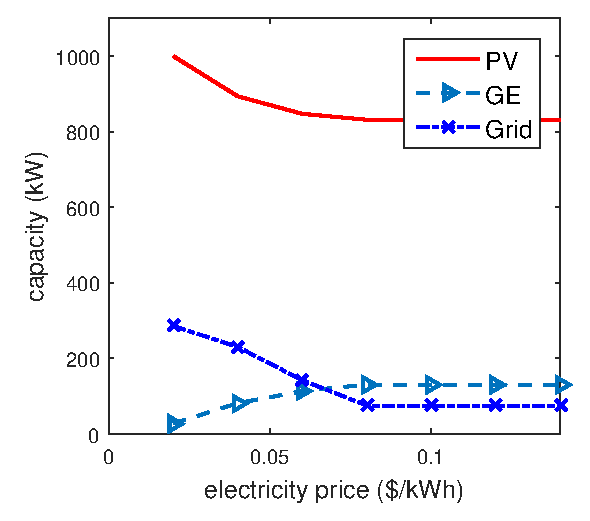
\includegraphics[width=0.32\columnwidth]{figs/capacity_electricity}}
		\label{f.capacity_electricity}}
	\subfigure[Payback period]{{\includegraphics[width=0.32\columnwidth]{figs/payback_electricity}}
		\label{f.payback_electricity}}
	\caption{Impacts of electricity prices. As the electricity price increases, the capacity of GE is increased to compensate for the PV generation during nighttime. Interestingly, it results in reducing the capacity of PV.}
	\label{f.electricity}
\end{center}
\vspace{-0.3cm}
\end{figure}
}

\emph{Electricity price}. Figure~\ref{f.electricity} presents the impacts of electricity prices on the proposed framework. Figure~\ref{f.capacity_electricity} shows that the data center uses more GE generation and less grid power when the electricity price increases. However, the data center surprisingly keeps reducing the capacity of PV. It is because the data center starts to use more GE to provide power during nighttime and replace PV during daytime. It is because the costs of GE are relatively lower than the infrastructure of PV as PV is not fully utilized around its peak generation. In addition, when the grid power becomes more expensive, the payback period sharply decreases as in Figure \ref{f.payback_electricity}. Hence, the NEDC can significantly gain financial benefits when the electricity prices are high.
\hideit{
\begin{figure}[!ht]
%	\vspace{-0.3cm}
\begin{center}
	\subfigure[Capacity]{{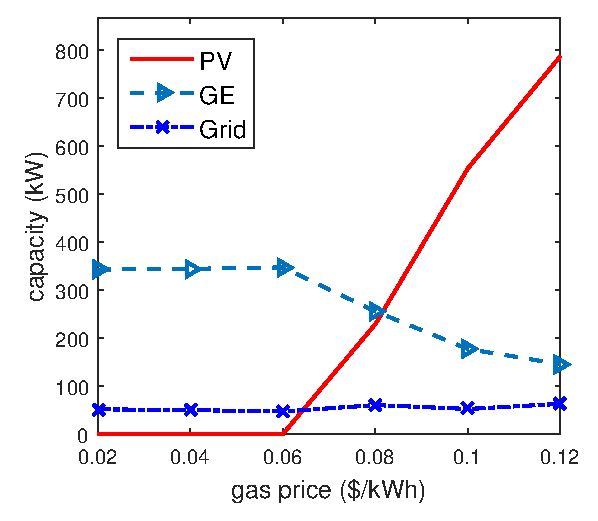
\includegraphics[width=0.32\columnwidth]{figs/capacity_gas}}
		\label{f.capacity_gas}}
	%        \subfigure[Cost]{{\includegraphics[width=0.48\columnwidth]{figs/cost_gas}}
	%            \label{f.cost_gas}}
	\subfigure[Payback period]{{
\includegraphics[width=0.32\columnwidth]{figs/payback_gas}}
		\label{f.payback_gas}}
 \vspace{-0.3cm}
	\caption{Impacts of gas prices. As the gas prices increase, the capacity of PV increases quickly because the data center cannot import too much electricity grid.}
	\label{f.gas}
\end{center}
\vspace{-0.3cm}
\end{figure}
}
\emph{Gas price.} Figure~\ref{f.gas} shows the impacts of gas prices on capacities and payback periods. In Figure \ref{f.capacity_gas}, the data center should use the GE generation at low gas prices, but it switches using PV when the gas price is more expensive. Especially, there is the sharp increase of PV capacity when the gas price is greater than $0.06$. Due to the non-dispatchability of solar energy, the data center needs the large capacity of PV generation to compensate for the reduction of GE generation. As the gas price increases, the payback period goes up as in Figure \ref{f.payback_gas} because the data center needs more PV.

\begin{figure}[!ht]
	%matlab: TCO_grid_payback_pv.m or TCO_grid_surface.m
	\begin{center}
		\subfigure[Capacity]{{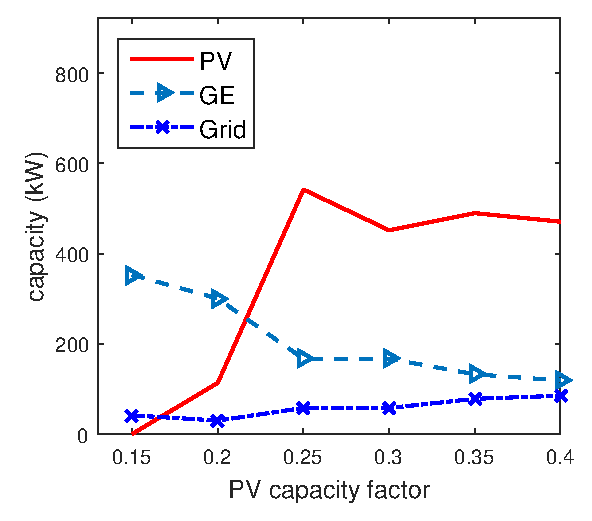
\includegraphics[width=0.32\columnwidth]{figs/capacity_PV}}
			\label{f.capacity_PV}}
		%        \subfigure[Cost]{{\includegraphics[width=0.48\columnwidth]{figs/cost_PV}}
		%            \label{f.cost_PV}}
		\subfigure[Payback period]{{\includegraphics[width=0.32\columnwidth]{figs/payback_PV}}
			\label{f.payback_PV}}
		\caption{Impact of different PV capacity factors. The curves of PV are very interesting which goes up and down because the high capacity factors have strong impact on the capital cost and operational cost of PV.}
		\label{f.PV}
	\end{center}
\end{figure}

\new{
	\emph{PV capacity factor.} To understand how PV capacity factors affect on the proposed framework, we run the experiments with various capacity factors of PV.
	Recall the capacity factor is the average power generated, divided by the rated peak power. Figure {\ref{f.PV}} shows the dependence of the capacities and payback periods of the data center on PV capacity factors. The capacity of PV increases and then varies at high capacity factors. The capacity factor of PV array varies due to diverse reasons, such as geographical conditions. When PV has enough efficiency, i.e. capacity factor varies from 0.15 to 0.25, the data center starts to use PV. At a very high capacity factor (0.25-0.4), it is not necessary to increase the PV capacity because even the lower capacity with high capacity factors can still provide enough generation.}

\textbf{\textit{Key insight}}: The capacities of PV, GE, and peak power of grid power consumption adapt to the variety of supply factors accordingly. (i) The impacts of electricity prices and gas prices show the trade-offs between PV and GE. (ii) Under the increase of electricity price, the capacity of PV unexpectedly goes down together with the peak grid power.	(iii) Under a certain gas price, the data center does not provision PV generation but only use GE and grid power instead.\delete{(iii) The impacts of PV capacity factors are complicated. Even at very high capacity factors, other power sources like GE and electricity grid play a crucial role to additionally supply the data center because PV is not available during nighttime.}

%%%%%%%%%%%%%%%%%%%%%%%%%%%%%%%%%%%%%%%%%%%%%%%%%%%%%%%%%%%%%%%%%%%%%%%%%%%%%%%%%%%%%%%%

\subsubsection{Impacts of demand factors.}

Besides the supply factors, it must be interesting to study how the demand factors impact on capacity planning and costs of the data center.
\hideit{
\begin{figure}[!ht]
	\vspace{-0.3cm}
	%matlab: TCO_grid_payback_PMR.m
	\begin{center}
		\subfigure[Capacity]{{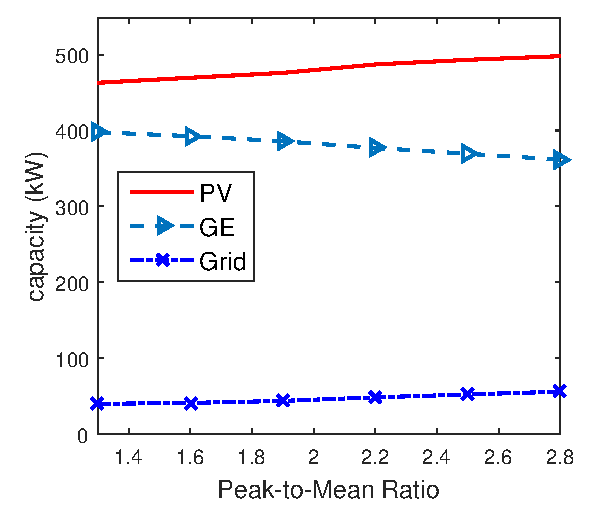
\includegraphics[width=0.32\columnwidth]{figs/capacity_PMR}}
			\label{f.capacity_PMR}}
		\subfigure[Cost]{{\includegraphics[width=0.32\columnwidth]{figs/cost_PMR}}
			\label{f.cost_PMR}}
		%\subfigure[Payback period]{{\includegraphics[width=0.48\columnwidth]{figs/payback_PMR}}
		\caption{Impacts of interactive workload shapes. The shapes of interactive workload have limited impacts on the capacities and expenditures of GE and PV.}
		\label{f.PMR}
	\end{center}
 \vspace{-0.3cm}
\end{figure}
}

\emph{Shape of interactive workload:} Interactive workload is non-flexible and required to be processed with high responsive speed in data centers. We use the peak-to-mean ratio (PMR) to study the impacts of interactive workload shape. Figure \ref{f.PMR} shows that shape of interactive workload has limited influence on both the capacities and expenditures of data centers. In particular, the capacity of PV and the peak grid power consumption slightly increase as the PMR increases. On the other hand, the data center slightly reduces GE when it has more PV power generation. As the capacities of PV and GE do not vary much, the breakdown expenditures are almost the same when varying the PMRs in Figure {\ref{f.cost_PMR}}.

\hideit{
\begin{figure}[!ht]
%matlab: TCO_grid_payback_ratio.m
\begin{center}
	\subfigure[Capacity]{{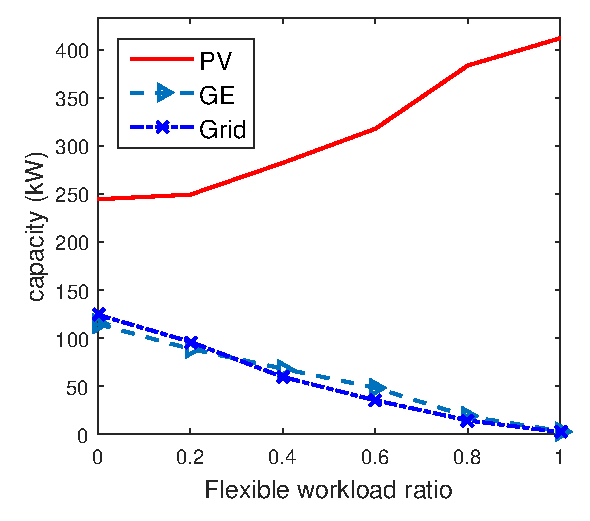
\includegraphics[width=0.32\columnwidth]{figs/capacity_batch}}
		\label{f.capacity_batch}}
	\subfigure[Cost]{{\includegraphics[width=0.32\columnwidth]{figs/cost_batch}}
		\label{f.cost_batch}}
	%\subfigure[Payback period]{{\includegraphics[width=0.48\columnwidth]{figs/payback_batch}}
	%\label{f.payback_batch}}
	\caption{Impacts of flexible workload ratios. The ratio can significantly reduces the total expenditure and change the capacity structure of the data center.}
	\label{f.batch_ratio}
\end{center}
\end{figure}
}
\emph{Ratio of flexible workload} is the ratio of batch jobs to the IT workload demand. The higher ratio of flexible workload means the more flexibility data centers have in power demand management. In particular, Figure~\ref{f.capacity_batch} highlight that the data center is more aggressive in using renewable energy as the ratio of flexible workload increases. It shows that the flexible workloads can promote the use of renewable sources. Especially, when workloads are totally flexible, there is no need to use GE and grid power as the workloads can be scheduled to totally follow PV generation. Figure~\ref{f.cost_batch} shows that the flexible workloads can significantly reduce the total expenditure, e.g., 28\% reduction of the total cost.

\textbf{\textit{Key insights}}: (i) The shape of interactive workload does not affect much on the capacity planning and operational management of data centers. (ii) The flexible workloads promote the use of renewable energy and significantly reduces the total cost.